\documentclass[12pt, letterpaper]{book}
\usepackage{graphicx} %LaTeX package to import graphics
\graphicspath{{../Immagini}} %configuring the graphicx package
\usepackage[T1]{fontenc}
\usepackage[italian]{babel}
\usepackage{hyphenat}
\hyphenation{mate-mati-ca recu-perare}
\usepackage{array}
\usepackage{booktabs} % Per linee orizzontali migliori
\usepackage{siunitx}  % Per formattare le unità di misura
\usepackage{caption}  % Per personalizzare le didascalie
\usepackage{multirow} % Per combinare celle nelle colonne
\usepackage{float}
\usepackage{hyperref}

%Domande:
%1) nei dispositivi che stiamo studiando il body è cortocircuitato con il source? 

% grafici che rappresentano l'andamaneto delle Vth al variare di W e L con i tre metodi 
% 

\begin{document}



\chapter{Estrazione dei parametri statici}

\section{Tensione di soglia}

La tensione di soglia $V_{th}$ di un transistore MOS è definita come quella tensione tra gate e bulk per la quale la popolazione di minoritari all'interfaccia è uguale alla popolazione di maggioritari nel bulk. Questa definizione non può essere usata direttamente per il calcolo della tensione di soglia dei dispositivi, ma si deve passare attraverso l'analisi delle caratteristiche corrente-tensione dei dispositivi. \\
Per l'estrazione del parametro $V_{th}$ esistono numerosi metodi, ognuno con punti di forza e punti di debolezza diversi. La scelta di quale metodo utilizzare non è banale e per farla occorre analizzare le caratteristiche di ciascun metodo e confrontare i risultati che offrono. Per questo studio sono stati presi in considerazione:

\begin{itemize}
  \item \emph{Transconductance Change Method (TCM)};
  \item \emph{Second Difference of the Logarithm of the drain current Minimum method (SDLM)};
  \item \emph{Extrapolation in the Linear Region method (ELR)}.
\end{itemize}

Per il nostro studio, però, non si è tanto interessati al valore in sé della tensione di soglia dei dispositivi, quanto più a come questa varia all'aumentare dell'irragiamento. Dunque, per ogni metodo non ci si ferma all'estrazione della $V_{th}$ dei dispositivi non irraggiati, ma la si estrae anche per ogni fase di irraggiamento e, per ciascuno di questi, si calcola la $\Delta V_{th} = V_{th, Irraggiato}-V_{th, non Irraggiato}$. La scelta di quale metodo effettivamente usare per le analisi successive viene presa sulla qualità del parametro $\Delta V_{th}$.


\subsection{Transconductance Change Method}

Il \emph{Transconductance Change Method, TCM,} defiscisce la tensione di soglia come la tensione di gate $V_{GS}$ corrispondente al picco massimo della derivata della transconduttanza $g_m$ rispetto alla tensione di gate ($\frac{dg_m}{dV_ {GS}}$) ed è valido per bassi valori della tensione $V_{DS}$.\\
Questa definizione si basa sul fatto che, quando il dispositivo passa dalla regione di debole inversione alla regione di forte inversione, la dipendenza della corrente di drain ripetto a $V_{GS}$ passa dall'essere esponenziale all'essere quasi constante.
La transconduttanza è definita come la derivata prima della corrente $I_D$ rispetto alla tensione $V_{GS}$, dunque la derivata della $g_m$ corrisponde alla derivata seconda di $I_D$. Per questo motivo, il massimo di $\frac{dg_m}{dV_{GS}}$ coincide con la tensione alla quale il grafico della corrente passa dalla forma esponenziale a quella quasi constante, ovvero la tensione $V_{GS}+V_{DS}$. Se $V_{DS}$ è piccola, la tensione per la quale la $g_m$ è massima è molto simile a $V_{th}$.\\

\begin{figure}[h!]
  \centering
  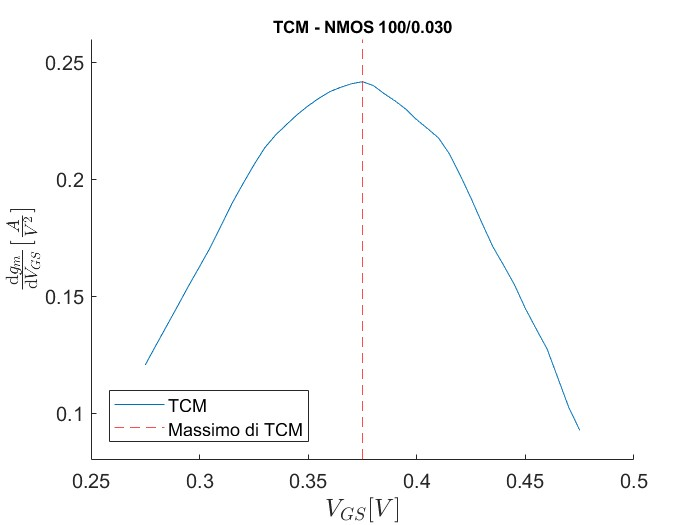
\includegraphics[width=0.49\textwidth]{TCM-N4-100-30-NoFit}
  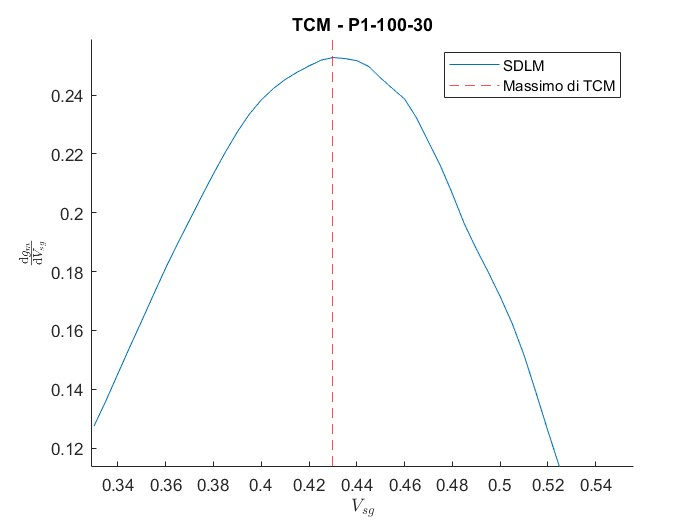
\includegraphics[width=0.49\textwidth]{TCM-P1-100-30-NoFit}
  \caption{Esempio di \emph{TCM} usato su un dispositivo NMOS e un dispositivo PMOS di dimensioni 100-30 a $V_{DS} = 150 mV$}
\end{figure}

\emph{TCM}, poiché si basa sul massimo di una funzione, è molto sensibile ai picchi dovuti ad errori di misura e perciò non è molto affidabile: è quindi necessario rendere la funzione studiata meno dipendente dai campionamenti fuori scala. Inoltre, la risoluzione del dispositivo di misura utilizzato e di $5 mV$, il che rende i valori ottenuti della $V_{th}$ molto approssimativi.
Per far fronte a questi due problemi, si è scelto di non tenere conto del massimo direttamente ottenuto dallo studio di $\frac{dg_m}{dV_{GS}}$ ottenuto dai valori delle misure, ma di interpolare prima i punti del grafico con una funzione polinomiale e, solo a questo punto, di prendere in considerazione il picco di massimo. \\

\begin{figure}[H]
  \centering
  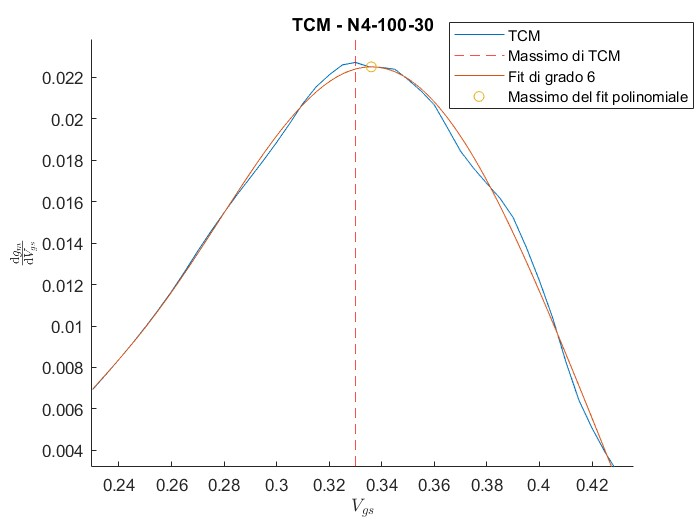
\includegraphics[width=0.49\textwidth]{TCM-N4-100-30}
  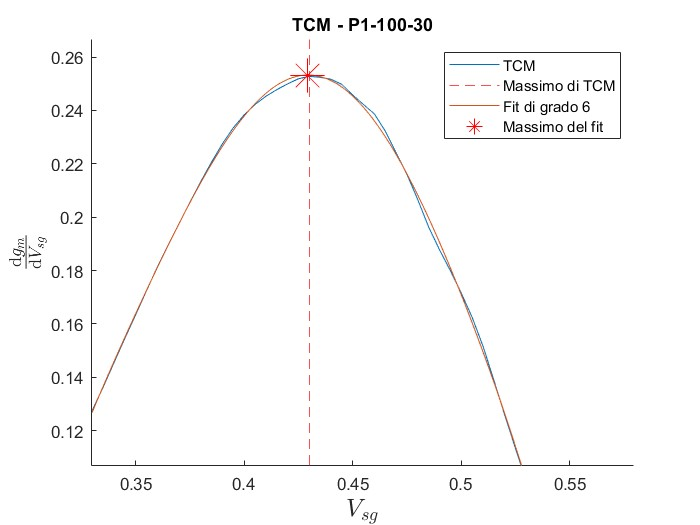
\includegraphics[width=0.49\textwidth]{TCM-P1-100-30}
  \caption{Esempio di \emph{TCM} con fit polinomiale usato su un dispositivo NMOS e un dispositivo PMOS di dimensioni 100-30 a $V_{DS} = 150 mV$}
\end{figure}

Lo studio del fit polinomiale risolve il problema della bassa risolizione di misura e il problema della presenza di valori fuori scala, ma presenta una potenziale nuovo problema: il valore della $V_{th}$ calcolata potrebbe variare significativamente al variare del grado della funzione polinomiale interpolante. Questa differenza non è molto alta, si parla di pochi millivolt, perciò non influenza considerevolmente il valore della singola estrazione. Questa dipendenza, però, è problematica nel momento in cui si vuole studiare con precisione la degradazione delle prestazioni di un dispositivo all'aumentare dell'irraggiamento subito, in quanto piccoli spostamenti del valore di $V_{th}$ dovuti alla scelta arbitraria del grado della polinomiale può far variare eccessivamente le differenze delle misure tra un irraggiamento e l'altro, elemento inaccettabile se si considera che già le misure sono influenzate da errori casuali in fase di misura.\\
Prendendo come esempio i dispositivi PMOS, si è studiato quanto cambia il valore della tenzione di soglia al variare del grado del fit polinomiale, prendendo in considerazione i gradi di valore 2, 4, 6 e 8.\\

\begin{table}[h]
  \renewcommand{\arraystretch}{1.3}
  \centering
  \begin{tabular}{m{2cm} m{2cm} m{2cm} m{2cm} m{2cm}}
    \toprule
    \multirow{2}{*}{Dispositivo} & \multicolumn{4}{c}{$V_{th} [mV] \text{ con grado:}$}                         \\
    \cmidrule{2-5}
                                 	& 2      		& 4     		& 6     		& 8     \\
    \midrule
    100 - 30                     	& 426.9   	& 429.4 		& 429.4 		& 430.8 \\
    \hline
    100 - 60                     	& 467.6    	& 469.5 		& 469.3 		& 468.9 \\
    \hline
    200 - 30                     	& 397.8  	 & 399.7   	& 399.3   	& 399.8   \\
    \hline
    200 - 60                    	& 452.2   	& 454.1   	& 453.5   	& 453.5   \\
    \hline
    200 - 180                     	& 495.6   	& 495.6   	& 495.3   	& 495.5   \\
    \hline
    600 - 30                     	& 383.0   	& 387.4   	& 385.9   	& 386.2   \\
    \hline
    600 - 60                    	& 431.1   	& 434.3   	& 434.7   	& 435.6   \\
    \hline
    600 - 180                   	& 478.5  	 & 480.8   	& 480.6   	& 480.0   \\
   
    \bottomrule
  \end{tabular}
  \caption{Confronto dei valori di $V_{th}$ dei dispositivi PMOS ottenuti con \emph{TCM} con fit polinomiale di diversi gradi}
  \label{tab:GradiTCM}
\end{table}

Osservando i valori nella tabella \ref{tab:GradiTCM}, si può notare che la tensione di soglia ottenuta non varia molto nel caso dei fit fatti con polinomiali di grado 4, 6 e 8: è raro che la differenza tra questi valori superi $1 mV$. Non si può dire la stessa cosa per le $V_{th}$ calcolate con fit di grado 2: in questo caso la funzione interpolante ha un grado troppo basso per seguire in modo coerente la curva $\frac{dg_m}{dV_{GS}}$ e quindi il massimo risulta essere sia molto diverso da quelli calcolati con fit di grado maggiore, sia da quello di ottenuto senza fit. Dunque di sicuro usare un fit di grado 2 porta a risultati scorretti, mentre usare un fit di grado superiore dovrebbe portare a risultati sicuramente accettabili. Per il confronto con altri metodi per l'estrazione della $V_{th}$ si terrà quindi conto del TCM con fit polinomiale di grado 6, tabelle \ref{tab:VthTCMP} e \ref{tab:VthTCMN}.


\begin{table}[H]
  \renewcommand{\arraystretch}{1.3}
    \begin{tabular}{m{2cm} m{0.8cm} m{1.1cm} m{1.3cm} m{1.5cm} m{1.5cm} m{1.5cm} m{1cm}}
      \toprule
      \multirow{2}{*}{Dispositivo} & \multicolumn{7}{c}{$V_{th} [mV] $}                                                                    \\
      \cmidrule{2-8}
                                   & pre                               & $5Mrad$ & $50Mrad$ & $100Mrad$ & $200Mrad$ & $600Mrad$ & $1Grad$ \\
      \midrule
      100 - 30               	& 429.4                             & 430.7   & 432.2    & 434.4     & 439.0     & 452.6     & 459.4   \\
      \hline
      100 - 60                 	& 469.3                             & 469.6   & 471.4    & 472.7     & 479.7     & 491.8     & 500.8   \\
      \hline
      200 - 30                  	& 399.3                             & 401.0   & 403.1    & 404.8     & 410.2     & 422.3     & 429.8   \\
      \hline
      200 - 60                    & 453.5                             & 455.2   & 456.2    & 458.6     & 463.8     & 476.9     & 485.8   \\
      \hline
      200 - 180 			& 495.3                             & 497.1   & 503.9    & 506.5     & 511.3     & 524.1     & 535.3   \\
      \hline
      600 - 30                  	& 385.9                             & 386.6   & 388.8    & 391.0     & 394.5     & 405.5     & 412.3   \\
      \hline
      600 - 60                    & 434.7                             & 435.4   & 438.5    & 438.9     & 445.6     & 458.4     & 467.8   \\
      \hline
      600 - 180              	& 480.6                             & 481.5   & 483.7    & 486.0     & 492.0     & 507.2     & 519.6   \\
      \bottomrule
    \end{tabular}
  \caption{$V_{th}$ dei dispositivi PMOS estratte con \emph{TCM}}
  \label{tab:VthTCMP}
\end{table}


\begin{table}[H]
  \renewcommand{\arraystretch}{1.3}
  \begin{tabular}{m{2cm} m{0.8cm} m{1.1cm} m{1.3cm} m{1.5cm} m{1.5cm} m{1.5cm} m{1cm}}
    \toprule
    \multirow{2}{*}{Dispositivo} & \multicolumn{7}{c}{$V_{th} [mV] $}                                                                    \\
    \cmidrule{2-8}
                                 & pre                                & $5Mrad$ & $50Mrad$ & $100Mrad$ & $200Mrad$ & $600Mrad$ & $1Grad$ \\
    \midrule
    100 - 30                     & 371.3                              & 370.6   & 361.0    & 380.6     & 378.7     &           &         \\
    \hline
    100 - 60                     & 405.0                              & 399.9   & 390.0    & 419.8     & 418.8     &           &         \\
    \hline
    100 - 180                    & 476.0                              & 472.4   & 459.5    & 491.9     & 491.2     &           &         \\
    \hline
    200 - 30                     & 359.5                              & 357.9   & 348.1    & 369.2     & 367.0     &           &         \\
    \hline
    200 - 60                     & 402.2                              & 398.3   & 385.0    & 415.5     & 413.7     &           &         \\
    \hline
    200 - 180                    & 466.4                              & 463.5   & 451.8    & 484.6     & 483.8     &           &         \\
    \hline
    600 - 60                     & 370.2                              & 364.4   & 359.3    & 379.5     & 381.0     &           &         \\
    \hline
    600 - 180                    & 449.6                              & 447.9   & 430.7    & 458.8     & 458.4     &           &         \\
    \bottomrule
  \end{tabular}
  \caption{$V_{th}$ dei dispositivi NMOS estratte con \emph{TCM}}
  \label{tab:VthTCMN}
\end{table}


\begin{table}[H]
  \renewcommand{\arraystretch}{1.3}
    \begin{tabular}{m{2cm}  m{1.1cm} m{1.3cm} m{1.5cm} m{1.5cm} m{1.5cm} m{1cm}}
      \toprule
      \multirow{2}{*}{Dispositivo} & \multicolumn{6}{c}{$V_{th} [mV] $}                                                                    \\
      \cmidrule{2-7}
                                   & $5Mrad$ & $50Mrad$ & $100Mrad$ & $200Mrad$ & $600Mrad$ & $1Grad$ \\
      \midrule
      100 - 30               	& 1.3   	& 2.8    	&  5.0    & 9.6     	& 23.2     	& 30.0   \\
      \hline
      100 - 60                 	& 0.3   	& 2.1    	& 3.4     & 10.4    	& 22.5     	& 31.5   \\
      \hline
      200 - 30                  	& 1.7   	& 3.8  	& 5.5     & 10.9    	&  23.0    	& 30.5   \\
      \hline
      200 - 60                    & 1.7   	& 2.7   	& 5.1     & 10.3   		& 23.4     	& 32.3  \\
      \hline
      200 - 180 			& 1.8   	& 8.6    	& 11.2   & 16.0   		& 28.8    	& 40.0   \\
      \hline
      600 - 30                  	& 0.7   	& 2.9    	& 5.1     &  8.6   		& 19.6     	& 26.4   \\
      \hline
      600 - 60                    & 0.7   	& 3.8    	& 4.2     & 10.9    	&  23.7    	& 33.1  \\
      \hline
      600 - 180              	& 0.9  	& 3.1    	& 5.4     & 11.4    	& 26.6     	&39.0   \\
      \bottomrule
    \end{tabular}
  \caption{$\Delta V_{th}$ dei dispositivi PMOS estratte con \emph{TCM}}
  \label{tab:deltaVthTCMP}
\end{table}

\begin{table}[H]
  \renewcommand{\arraystretch}{1.3}
    \begin{tabular}{m{2cm}  m{1.1cm} m{1.3cm} m{1.5cm} m{1.5cm} m{1.5cm} m{1cm}}
      \toprule
      \multirow{2}{*}{Dispositivo} & \multicolumn{6}{c}{$V_{th} [mV] $}                                                                    \\
      \cmidrule{2-7}
                                   & $5Mrad$ & $50Mrad$ & $100Mrad$ & $200Mrad$ & $600Mrad$ & $1Grad$ \\
      \midrule
      100 - 30               	& -0.7		& -10.3		& 9.3		& 7.4		& 3.8		&    \\
      \hline
      100 - 60                 	& -5.1		& -15.0		& 14.8		& 13.8		& 9.0		&    \\
      \hline
      200 - 30                  	& -3.6		& -16.5		& 15.9		&15.2		& 16.0		&    \\
      \hline
      200 - 60                    & -1.6		& -11.4		& 9.7		& 7.5		& 4.3		&   \\
      \hline
      200 - 180 			& -3.9		&  -17.2		& 13.3		& 11.5		& 10.1		&    \\
      \hline
      600 - 30                  	& -2.9   		& -14.6		& 18.2		& 17.4		& 20.1		&    \\
      \hline
      600 - 60                    & -5.8   		& -10.9		& 9.3		& 10.8		& 7.9		&   \\
      \hline
      600 - 180              	& -1.7  		& -18.9		& 9.2		& 8.8		& 9.3		&  \\
      \bottomrule
    \end{tabular}
  \caption{$\Delta V_{th}$ dei dispositivi NMOS estratte con \emph{TCM}}
  \label{tab:deltaVthTCMN}
\end{table}








\subsection{Second Difference of the Logarithm of the drain current Minimum method}

Il secondo metodo analizzato è il \emph{Second Difference of the Logarithm of the drain current Minimum method, SDLM}. Questo metodo definisce la $V_{th}$ come la tensione $V_{GS}$ per la quale si ha il picco minimo della derivata seconda del logaritmo naturale di $I_D$ ripetto alla tensione di gate ($\frac{d^2lnI_D}{dV_{GS}^2}$) e vale solo per alti valori di $V_{DS}$. \\

\begin{figure}[H]
  \centering
  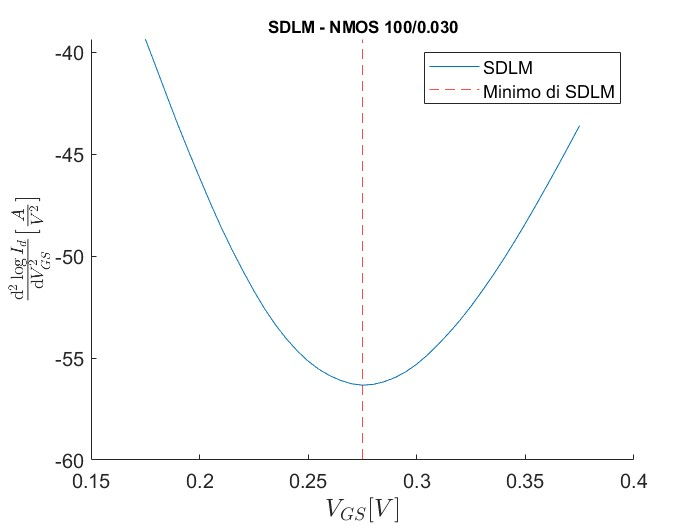
\includegraphics[width=0.49\textwidth]{SDLM-N4-100-30-NoFit}
  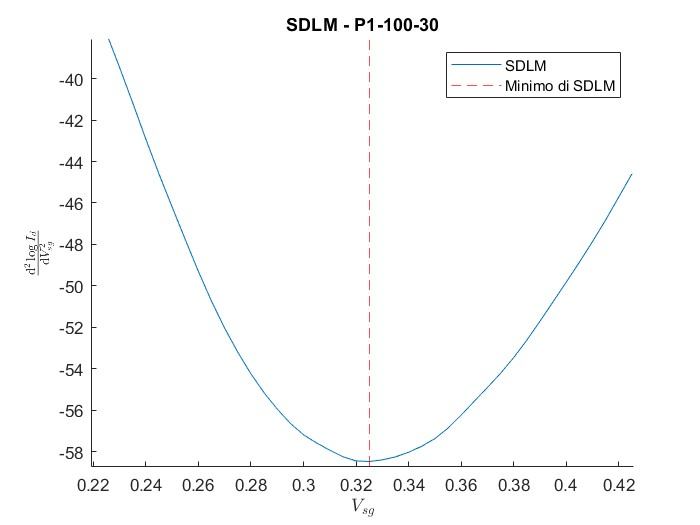
\includegraphics[width=0.49\textwidth]{SDLM-P1-100-30-NoFit}
  \caption{Esempio di \emph{SDLM} usato su un dispositivo NMOS e un dispositivo PMOS di dimensioni 100-30 a $V_{DS} = 900 mV$}
\end{figure}


Anche per questo metodo si ritovano le problematiche presenti per il \emph{TCM}: il valore minimo della funzione analizzata è fortemente influenzata dai valori fuori scala e la risoluzione dello strumento di misura è di $5 mV$ e dunque troppo grossolana per ottenere un valore preciso di $V_{th}$.
Quindi, anche per questo metodo, abbiamo deciso di interpolare la funzione ottenuta con una polinomiale e considerare il minimo di quest'ultima. \\

\begin{table}[htp] 
\renewcommand{\arraystretch}{1.3}
\caption{Confronto dei valori di $V_{th}$ dei dispositivi PMOS ottenuti con \emph{SDLM} con fit polinomiale di diversi gradi}
\label{tab:GradiSDLM} 
\begin{center}
\begin{tabular}{c c c c c}
\hline
Dispositivo &  $V_{th}$  con fit di & $V_{th}$  con fit di & $V_{th}$  con fit di & $V_{th}$  con fit di \\
 & grado 2 $[mV]$ & grado 4 $[mV]$ & grado 6 $[mV]$ & grado 8 $[mV]$ \\
\hline
100 - 30  & 332.0 & 322.3 & 323.5 & 327.2 \\
\hline
100 - 60  & 423.1 & 416.1 & 411.6 & 411.7 \\
\hline
200 - 30  & 303.2 & 298.8 & 296.5 & 296.7 \\
\hline
200 - 60 & 413.1 & 404.4 & 404.9 & 405.0 \\
\hline
200 - 180  & 460.4 & 453.5 & 449.3 & 448.7\\
\hline
600 - 30 & 296.0 & 291.4 & 289.7 & 298.1 \\
\hline
600 - 60 & 398.3 & 393.3 & 391.8 & 389.6 \\
\hline
600 - 180 & 454.7  & 446.7 & 441.4 & 441.3 \\
\hline
\end{tabular}
\end{center}
\end{table} 



\begin{figure}[h!]
  \label{fig:GradiSDLM}
  \centering
  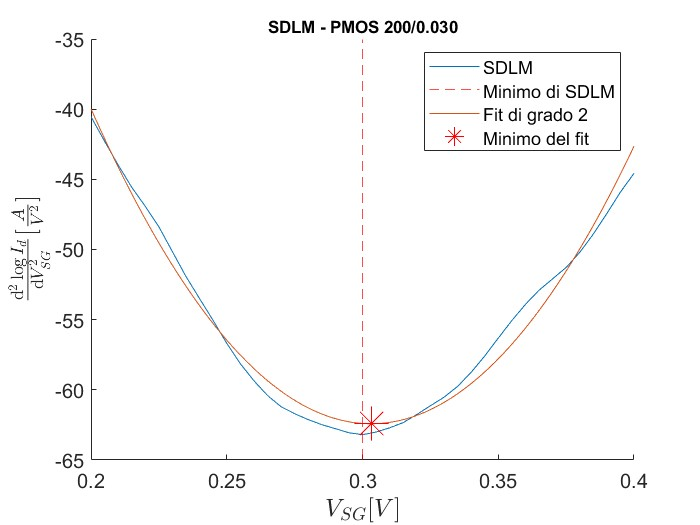
\includegraphics[width=0.49\textwidth]{SDLM-P1-200-30-grado2}
  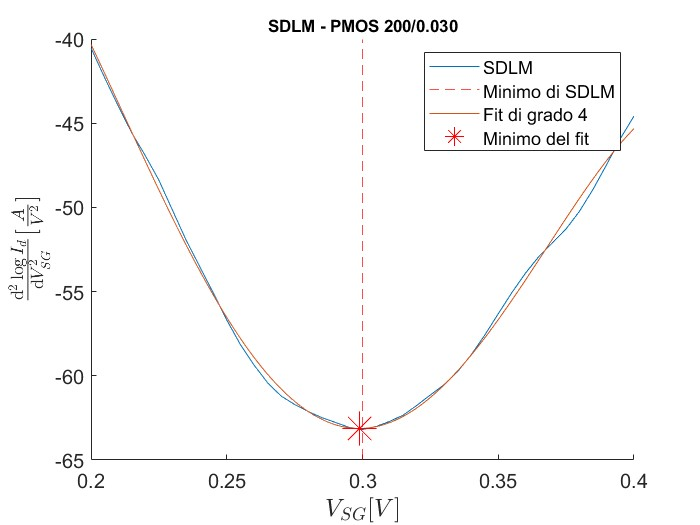
\includegraphics[width=0.49\textwidth]{SDLM-P1-200-30-grado4}
  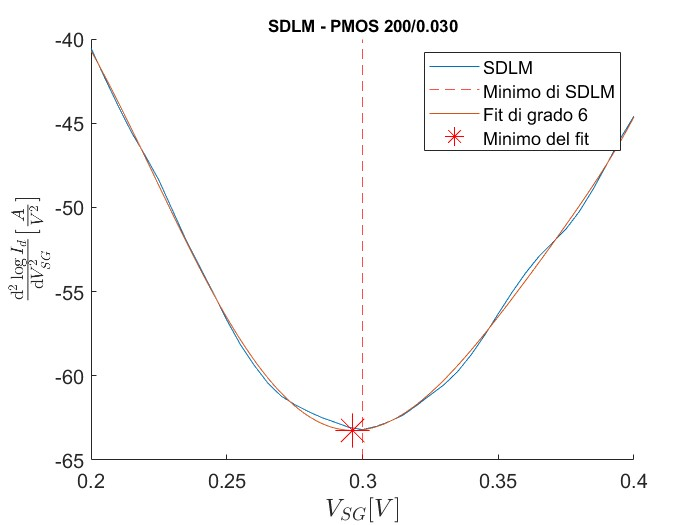
\includegraphics[width=0.49\textwidth]{SDLM-P1-200-30-grado6}
  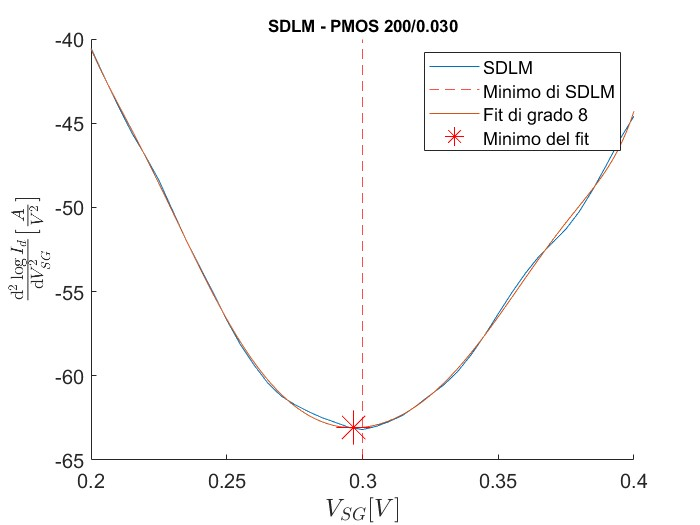
\includegraphics[width=0.49\textwidth]{SDLM-P1-200-30-grado8}
  \caption{Confronto dei valori di $V_{th}$ del dispositivo PMOS 200-30 ottenuti con \emph{SDLM} con fit polinomiale di diversi gradi}
\end{figure}

Prendendo in considerazione i dati presenti nella tabella \ref{tab:GradiTCM}, si nota come $V_{th}$ assume valori molto diversi a seconda del grado della polinomiale interpolante. Nella maggior parte dei casi, le tensioni di soglia ottenute con polinomiali di grado basso (2 e 4) cambiano molto tra loro e rispetto a quelle ottenute con polinomiali di grado alto (6 e 8), metre le misure ottenute con quete ultime sono, in genere, molto simili tra loro. Osservando i grafici relativi alla SDLM del PMOS 200-30 (figura \ref{fig:GradiTCM}), si può nota che il plot della funzione $\frac{d^2lnI_D}{dV_{GS}^2}$ ha un andamento che non viene interpolato in modo preciso da polinomiali di basso grado: per questo i valori minimi si discostano parecchio dai minimi ottenuti con polinomiali di grado maggiore. Risulta, infatti, che \emph{SDLM} è più sensibile agli errori di misurazioni rispetto a \emph{TCM} e quindi i grafici sono meno approssimabili a polinomiali di baso grado. Si ha dunque che:
\begin{itemize}
  \item I fit di grado basso non interpolano in modo preciso il grafico di $\frac{d^2lnI_D}{dV_{GS}^2}$ i valori minimi variano considerevolmente al variare del grado.
  \item I fit di grado alto interpolano bene il grafico di partenza e i valori minimi sono simili tra loro, ma influenzati dagli errori di misura
\end{itemize}

Non è quindi semplice capire quale grado usare per interpolare $\frac{d^2lnI_D}{dV_{GS}^2}$ e, in generale, abbiamo concluso che questo metodo non pare molto affidabile per questo studio. In ogni caso, per i futuri confronti tra i metodi si terrà lo stesso in conto l'\emph{SDLM}, usando un fit di grado 6, che può essere considerata un'accettabile via di mezzo tra le polinomiali che non interpolano bene il grafico di partenza e quelle che sono troppo influenzate dagli errori di misura.


\begin{table}[H]
  \renewcommand{\arraystretch}{1.3}
  \begin{tabular}{m{2cm} m{0.8cm} m{1.1cm} m{1.3cm} m{1.5cm} m{1.5cm} m{1.5cm} m{1cm}}
    \toprule
    \multirow{2}{*}{Dispositivo} & \multicolumn{7}{c}{$V_{th} [mV] $}                                                                    \\
    \cmidrule{2-8}
                                 & pre                                & $5Mrad$ & $50Mrad$ & $100Mrad$ & $200Mrad$ & $600Mrad$ & $1Grad$ \\
    \midrule
    100 - 30                     & 323.5                              & 329.9   & 327.3    & 330.7     & 329.7     & 343.2     & 355.8   \\
    \hline
    100 - 60                     & 411.6                              & 409.9   & 412.3    & 415.5     & 416.8     & 428.3     & 435.8   \\
    \hline
    200 - 30                     & 296.5                              & 292.4   & 301.7    & 299.8     & 304.4     & 320.0     & 323.0   \\
    \hline
    200 - 60                     & 404.9                              & 403.9   & 405.3    & 407.3     & 413.0     & 422.5     & 430.9   \\
    \hline
    200 - 180                    & 449.3                              & 452.1   & 457.6    & 456.9     & 461.9     & 473.7     & 482.7   \\
    \hline
    600 - 30                     & 289.7                              & 293.0   & 297.3    & 297.0     & 299.9     & 313.1     & 325.7   \\
    \hline
    600 - 60                     & 391.8                              & 393.4   & 397.4    & 396.8     & 402.0     & 415.1     & 421.2   \\
    \hline
    600 - 180                    & 441.4                              & 443.4   & 445.1    & 444.6     & 450.9     & 464.5     & 474.2   \\
    \bottomrule
  \end{tabular}
  \caption{$V_{th}$ dei dispositivi PMOS estratte con \emph{SDLM}}
  \label{tab:VthSDLMP}
\end{table}


\begin{table}[H]
  \renewcommand{\arraystretch}{1.3}
  \begin{tabular}{m{2cm} m{0.8cm} m{1.1cm} m{1.3cm} m{1.5cm} m{1.5cm} m{1.5cm} m{1cm}}
    \toprule
    \multirow{2}{*}{Dispositivo} & \multicolumn{7}{c}{$V_{th} [mV] $}                                                                    \\
    \cmidrule{2-8}
                                 & pre                                & $5Mrad$ & $50Mrad$ & $100Mrad$ & $200Mrad$ & $600Mrad$ & $1Grad$ \\
    \midrule
    100 - 30                     & 287.7                              & 259.5   & 271.2    & 289.8     & 287.7     &           &         \\
    \hline
    100 - 60                     & 356.8                              & 327.2   & 322.7    & 360.9     & 356.8     &           &         \\
    \hline
    100 - 180                    & 404.8                              & 381.5   & 369.1    & 422.1     & 404.8     &           &         \\
    \hline
    200 - 30                     & 279.7                              & 262.2   & 269.6    & 277.9     & 279.7     &           &         \\
    \hline
    200 - 60                     & 355.3                              & 325.4   & 313.3    & 357.4     & 355.3     &           &         \\
    \hline
    200 - 180                    & 417.9                              & 378.9   & 372.5    & 418.8     & 417.9     &           &         \\
    \hline
    600 - 60                     & 334.4                              & 276.0   & 304.0    & 336.1     & 334.4     &           &         \\
    \hline
    600 - 180                    & 417.1                              & 381.5   & 379.6    & 418.4     & 417.1     &           &         \\
    \bottomrule
  \end{tabular}
  \caption{$V_{th}$ dei dispositivi NMOS estratte con \emph{SDLM}}
  \label{tab:VthSDLMN}
\end{table}


\begin{table}[H]
  \renewcommand{\arraystretch}{1.3}
    \begin{tabular}{m{2cm}  m{1.1cm} m{1.3cm} m{1.5cm} m{1.5cm} m{1.5cm} m{1cm}}
      \toprule
      \multirow{2}{*}{Dispositivo} & \multicolumn{6}{c}{$V_{th} [mV] $}                                                                    \\
      \cmidrule{2-7}
                                   & $5Mrad$ & $50Mrad$ & $100Mrad$ & $200Mrad$ & $600Mrad$ & $1Grad$ \\
      \midrule
	100 - 30				& 6.4		& 3.8		& 7.2		& 6.2		& 19.7		& 32.3\\
      \hline
      100 - 60				& -1.7		& 0.7		& 3.9		& 5.2		& 16.7		& 24.2   \\
      \hline
      200 - 30				& -4.1		& 5.2		& 3.3		& 7.9		& 23.5 		& 26.5  \\
      \hline
      200 - 60				& -1.0		& 0.4 		& 2.4		& 8.1		& 17.6		& 26.0  \\
      \hline
      200 - 180			& 2.8 		& 8.3		& 7.6		& 12.6		& 24.4		& 33.4   \\
      \hline
      600 - 30				& 3.3		& 7.6		& 7.3		& 10.2 		& 23.4		& 36.0   \\
      \hline
      600 - 60				& 1.6		&5.6 		& 5.0		& 10.2		& 23.3		& 29.4  \\
      \hline
      600 - 180			& 2.0		& 3.7		& 3.2		& 9.5		& 23.1		& 32.8   \\
      \bottomrule
    \end{tabular}
  \caption{$\Delta V_{th}$ dei dispositivi PMOS estratte con \emph{SDLM}}
  \label{tab:deltaVthSDLMP}
\end{table}

\begin{table}[H]
  \renewcommand{\arraystretch}{1.3}
    \begin{tabular}{m{2cm}  m{1.1cm} m{1.3cm} m{1.5cm} m{1.5cm} m{1.5cm} m{1cm}}
      \toprule
      \multirow{2}{*}{Dispositivo} & \multicolumn{6}{c}{$V_{th} [mV] $}                                                                    \\
      \cmidrule{2-7}
                                   & $5Mrad$		& $50Mrad$& $100Mrad$ & $200Mrad$ & $600Mrad$ & $1Grad$ \\
      \midrule
      100 - 30               	& -20.2		& -8.5		& 10.1		& 8.0		& -1.2		&    \\
      \hline
      100 - 60                 	& 12.1		& 7.6		& 45.8		& 41.7		& 41.5		&    \\
      \hline
      200 - 30                  	& 12.1		& -0.3		& 52.7		& 35.4		&52.7 		&    \\
      \hline
      200 - 60                    & -2.5		& 4.9		& 13.2		& 15.0		& 2.6		&   \\
      \hline
      200 - 180 			& -0.6		& -12.7 		& 31.4		& 29.3		& 25.1		&    \\
      \hline
      600 - 30                  	& 7.1		& 0.7		& 47.0		& 46.1		& 48.3		&    \\
      \hline
      600 - 60                    & -29.1  		& -1.1		& 31.0		& 29.3		& 27.6		&   \\
      \hline
      600 - 180              	& -3.3 		& --5.2		& 33.6		& 32.3		& 31.4		&  \\
      \bottomrule
    \end{tabular}
  \caption{$\Delta V_{th}$ dei dispositivi NMOS estratte con \emph{SDLM}}
  \label{tab:deltaVthSDLMN}
\end{table}








\subsection{Extrapolation in the Linear Region method}


Il terzo metodo analizzato è l'\emph{Extrapolation in the Linear Region method, ELR}, con il quale si ottiene la misura della $V_{th}$ attraverso l'analisi della caratteristica $I_D-V_{GS}$.  Tale grafico presenta un punto di flesso attorno al quale il grafico è linearizzabile. Il valore di $V_{th}$ si ottiene sommando la metà del valore di $V_{DS}$ al valore di $V_{GS}$ al quale il fit lineare, ottenuto nell'intorno del punto di flesso, interseca l'asse delle ascisse.\\


\begin{figure}[h!]
  \centering
  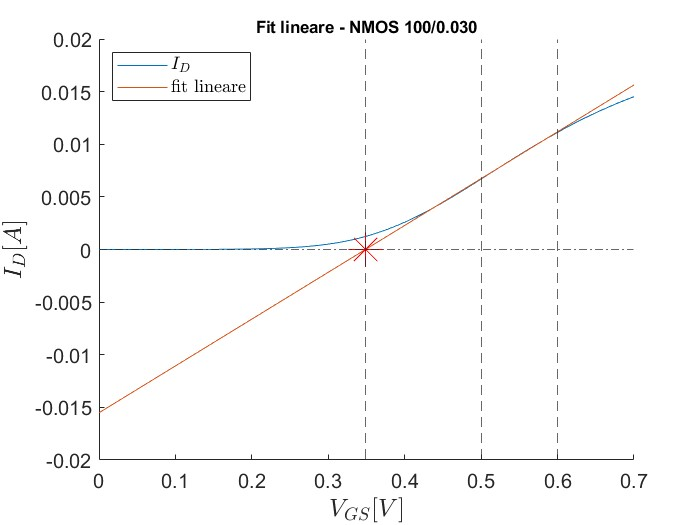
\includegraphics[width=0.49\textwidth]{LinearFit-N4-100-30}
  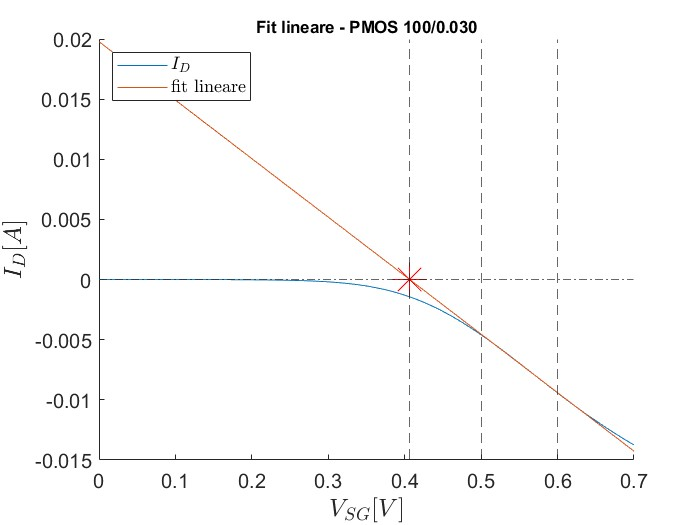
\includegraphics[width=0.49\textwidth]{LinearFit-P1-100-30}
  \caption{Fit lineare della caratteristica  $I_D$-$V_{GS}$ a $V_{DS}=150mV$ di un NMOS e di un PMOS di dimensioni 100-30 }
\end{figure}

Di per sé, questo metodo è meno preciso di quelli esposti precedentemente: la posizione del punto di flesso può essere incerto, perché, già a $V_{GS}$ leggermente superiori a $V_{th}$, la caratteristica $I_D-V_{GS}$ può deviare dall'andamento lineare previsto a causa di errori dovuti alle resistenze parassite presenti al source e al drain dei dispositivi e alla degradazione della mobilità dei portatori di carica.
Nonostante ciò, per il nostro studio questo metodo potrebbe risultare efficace, in quanto non siamo interessati al valore della tensione di soglia dei dispositivi, ma alla differenza di tale parametro all'aumentare dell'irraggiamento subito dai dispositivi. Dunque gli errori prodotti dalle resistenze parassite e dalla degradazione di mobilità divenatano irrilevanti, perché sono offset che vengono eliminati nel momento in cui si calcola la differenza tra due misure di $V_{th}$ dello stesso dispositivo.\\
È infine doveroso fare una parentesi sulla regione di linearizzazione considerata per questo studio: infatti non è possibile stabilire con certezza una regione fissa in cui la funzione, ottenuta con misure sperimentali, può essere linearizzata. Il metodo da noi applicato è stato quello di analizzare tutti i possibili intervalli di linearizzazione di dimensione $100 mV$ i cui estremi ricadono nell'intervallo $[300 mV ; 750mV]$ e scegliere quello il cui il fit approssimava meglio la funzione. All'atto pratico abbiamo considerato l'intervallo il cui fit ha il coefficiente di determinazione $R^2$ piu alto, che è risultato essere sempre maggiore di $0.999$.


\begin{table}[H]
  \renewcommand{\arraystretch}{1.3}
    \begin{tabular}{m{2cm} m{0.8cm} m{1.1cm} m{1.3cm} m{1.5cm} m{1.5cm} m{1.5cm} m{1cm}}
      \toprule
      \multirow{2}{*}{Dispositivo} & \multicolumn{7}{c}{$V_{th} [mV] $}                                                                    \\
      \cmidrule{2-8}
                                   	& pre  			& $5Mrad$ & $50Mrad$ & $100Mrad$ & $200Mrad$ & $600Mrad$ & $1Grad$ \\
      \midrule
      100 - 30                 	& 405.8      		& 406.6		& 408.6     	& 410.1 		& 416.1     	& 429.3     	& 436.6   \\
      \hline
      100 - 60                  	& 452.0            	& 452.9    	& 454.6    	& 456.5  	& 462.9     	& 475.4     	& 484.9   \\
      \hline
      200 - 30 			& 376.2          	& 377.6   	& 379.3   	& 380.3    	& 386.9     	& 397.5   	& 404.7   \\
      \hline
      200 - 60                  	& 434.6			& 435.9  	& 437.5    	& 439.3    	& 445.1   	& 458.1    	& 467.2   \\
      \hline
      200 - 180                 	& 482.3      		& 483.5   	& 490.3   	& 492.4    	& 498.5    	& 511.5     	& 522.6   \\
      \hline
      600 - 30               	& 359.4           	& 360.9		& 362.5    	& 364.6     	& 370.1     	& 379.8    	& 387.1   \\
      \hline
      600 - 60              	& 412.8           	& 414.2    	& 417.1   	& 417.5      	& 424.5    	& 437.3      	& 446.1   \\
      \hline
      600 - 180                	& 463.2            	& 464.4    	& 466.4   	& 468.9     	& 475.2     	& 490.8      	& 502.9   \\
      \bottomrule
    \end{tabular}

  \caption{$V_{th}$ dei dispositivi PMOS estratte con \emph{ELR}}
  \label{tab:VthELRP}
\end{table}


\begin{table}[H]
  \renewcommand{\arraystretch}{1.3}
  \begin{tabular}{m{2cm} m{0.8cm} m{1.1cm} m{1.3cm} m{1.5cm} m{1.5cm} m{1.5cm} m{1cm}}
    \toprule
    \multirow{2}{*}{Dispositivo} & \multicolumn{7}{c}{$V_{th} [mV] $}                                                                    \\
    \cmidrule{2-8}
                                 & pre                                & $5Mrad$ & $50Mrad$ & $100Mrad$ & $200Mrad$ & $600Mrad$ & $1Grad$ \\
    \midrule
    100 - 30                     & 351.0                              & 348.5   & 338.8    & 360.4     & 440.1     & 0.3531    &         \\
    \hline
    100 - 60                     & 388.8                              & 385.3   & 373.1    & 403.8     & 361.4     & 0.3988    &         \\
    \hline
    100 - 180                    & 465.9                              & 461.6   & 449.4    & 482.5     & 471.0     & 0.4823    &         \\
    \hline
    200 - 30                     & 336.9                              & 334.6   & 324.6    & 346.0     & 395.1     & 0.3413    &         \\
    \hline
    200 - 60                     & 382.9                              & 379.4   & 366.4    & 396.6     & 344.7     & 0.3934    &         \\
    \hline
    200 - 180                    & 454.6                              & 449.8   & 438.1    & 471.1     & 481.7     & 0.4736    &         \\
    \hline
    600 - 60                     & 349.3                              & 347.2   & 336.7    & 361.2     & 402.0     & 0.3581    &         \\
    \hline
    600 - 180                    & 431.8                              & 427.5   & 412.4    & 440.6     & 358.4     & 0.4408    &         \\
    \bottomrule
  \end{tabular}
  \caption{$V_{th}$ dei dispositivi NMOS estratte con \emph{ELR}}
  \label{tab:VthELRN}
\end{table}

\begin{table}[H]
  \renewcommand{\arraystretch}{1.3}
    \begin{tabular}{m{2cm}  m{1.1cm} m{1.3cm} m{1.5cm} m{1.5cm} m{1.5cm} m{1cm}}
      \toprule
      \multirow{2}{*}{Dispositivo} & \multicolumn{6}{c}{$V_{th} [mV] $}                                                                    \\
      \cmidrule{2-7}
                                   & $5Mrad$ & $50Mrad$ & $100Mrad$ & $200Mrad$ & $600Mrad$ & $1Grad$ \\
      \midrule
	100 - 30				& 0.8		& 2.8		& 4.4		& 10.4		& 23.5		& 30.8   \\
      \hline
      100 - 60				& 0.9		& 2.6		&4.5 		& 10.9		& 23.3		&  32.9  \\
      \hline
      200 - 30				& 1.4		& 3.2		& 4.1		& 10.8		& 21.3		& 28.6   \\
      \hline
      200 - 60				& 1.3		& 2.9		& 4.7		& 10.5		& 23.5		& 32.6  \\
      \hline
      200 - 180				& 1.2		& 8.0		& 10.1		& 16.2		& 29.3		& 40.4   \\
      \hline
      600 - 30				& 1.5		& 3.2		& 5.2		& 10.7  	& 20.4		& 27.7   \\
      \hline
      600 - 60				& 1.4		& 4.3		& 4.8		& 11.8		& 24.5 		& 33.3 \\
      \hline
      600 - 180				& 1.2		&3.2		& 5.7		& 12.0		& 27.6   	& 39.7 \\
      \bottomrule
    \end{tabular}
  \caption{$\Delta V_{th}$ dei dispositivi PMOS estratte con \emph{ELR}}
  \label{tab:deltaVthELRP}
\end{table}

\begin{table}[H]
  \renewcommand{\arraystretch}{1.3}
    \begin{tabular}{m{2cm}  m{1.1cm} m{1.3cm} m{1.5cm} m{1.5cm} m{1.5cm} m{1cm}}
      \toprule
      \multirow{2}{*}{Dispositivo} & \multicolumn{6}{c}{$V_{th} [mV] $}                                                                    \\
      \cmidrule{2-7}
                                   & $5Mrad$		& $50Mrad$& $100Mrad$ & $200Mrad$ & $600Mrad$ & $1Grad$ \\
      \midrule
      100 - 30               	& -2.5		& -12.1		& 9.4		& 7.4		& 2.1		&    \\
      \hline
      100 - 60                 	& -3.5		& -15.8		& 15.0		& 13.1		& 10.0		&    \\
      \hline
      200 - 30                  	& -4.3		& -16.5		& 16.6		&15.8		& 16.3		&    \\
      \hline
      200 - 60                    & -2.3		& -12.3		& 9.1		& 7.9		& 4.5		&   \\
      \hline
      200 - 180 			& -3.5		& -16.5 		& 13.6		&12.2		& 10.5		&    \\
      \hline
      600 - 30                  	& -4.9		& -16.5		& 16.5		& 16.4		& 19.1		&    \\
      \hline
      600 - 60                    & -2.2  		& -12.7		& 11.8		& 12.0		& 8.8		&   \\
      \hline
      600 - 180              	& -4.3  		& -19.4		& 8.8		& 8.2		& 9.0		&  \\
      \bottomrule
    \end{tabular}
  \caption{$\Delta V_{th}$ dei dispositivi NMOS estratte con \emph{ELR}}
  \label{tab:deltaVthELRN}
\end{table}






\subsection{Ratio Method}

Il \emph{Ratio Method, RM} è stato sviluppato per far fronte alle problematicità dell'\emph{ELR}: è stato infatti dimostrato che questo metodo non è influenzato dalla degradazione della mobilità dei portatori di carica né dalle correnti parassite. Questo metodo si basa sull'assunzione che, a bassi valori di tensione di drain $V_{DS}$, il rapporto tra la corrente di drain $I_D$ e la radice quadrata della transcondutanza $g_m$ ($\frac{I_D}{g_m^{0.5}}$) in funzione della tensione di gate $V_{GS}$ si comporti come una funzione lineare. La tensione di soglia $V_{th}$ coincide con il valore della tensione $V_{GS}$ a cui la funzione interseca l'asse della ascisse. \\
Come detto, questo metodo supera alcuni limiti dei metodi descritti in precedenza, però presenta una problematicità non indifferente: tracciando il grafico di $\frac{I_D}{g_m^{0.5}}$ in funzione di $V_{GS}$, questo non verifica appieno l'assunzione di linearità. Dunque non esiste un intervallo in cui il grafico è chiaramente linearizzabile e quindi la misura di $V_{th}$ non rispecchia del tutto il valore reale della tensione di soglia, ma è comunque una buona approssimazione, soprattutto se si considera il $\Delta V_{th}$ al crecere dell'irraggiamento.\\
Anche il questo caso, per ottenere il fit lineare più accurato possibile è stato usato lo stesso metodo esposto per l'\emph{ELR}.


\begin{figure}[h!]
  \centering
  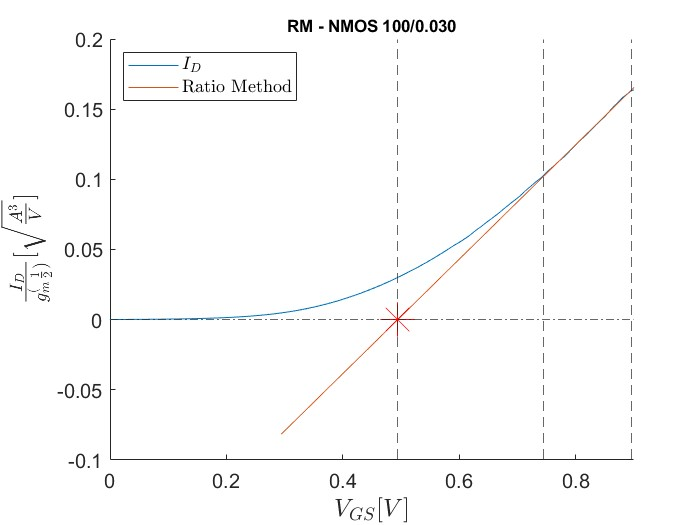
\includegraphics[width=0.49\textwidth]{RM-N4-100-30}
  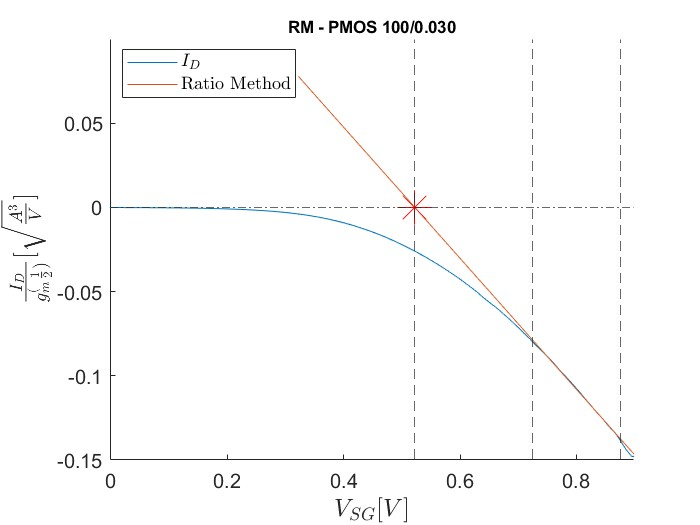
\includegraphics[width=0.49\textwidth]{RM-P1-100-30}
  \caption{Fit lineare della caratteristica $\frac{I_D}{g_m^{0.5}}-V_{GS}$ a $V_{DS}=150mV$ di un NMOS e di un PMOS di dimensioni 100-30}
\end{figure}

\begin{table}[H]
  \renewcommand{\arraystretch}{1.3}
    \begin{tabular}{m{2cm} m{0.8cm} m{1.1cm} m{1.3cm} m{1.5cm} m{1.5cm} m{1.5cm} m{1cm}}
      \toprule
      \multirow{2}{*}{Dispositivo} & \multicolumn{7}{c}{$V_{th} [mV] $}                                                                    \\
      \cmidrule{2-8}
                                   	& pre  			& $5Mrad$ & $50Mrad$ & $100Mrad$ & $200Mrad$ & $600Mrad$ & $1Grad$ \\
      \midrule
      100 - 30                 	& 522.3     		& 529.8		& 530.7    	& 532.2 		&  533.3    	& 544.4     	& 547.3   \\
      \hline
      100 - 60                  	& 543.6            	& 543.3    	& 541.8   	& 545.4  	& 548.9     	& 528.1     	& 541.6   \\
      \hline
      200 - 30 			& 525.2          	& 520.5   	& 527.4  	& 542.2   	& 544.8     	& 551.1   	& 554.7   \\
      \hline
      200 - 60                  	&547.9			& 540.5 		& 549.1    	& 550.6   	& 555.7   	& 563.1    	& 568.3   \\
      \hline
      200 - 180                 	& 551.1      		& 553.1    	& 538.3  	&538.0     	& 545.0    	& 568.8    	& 576.8   \\
      \hline
      600 - 30               	& 527.8           	& 539.9		& 537.3   	& 540.2     	& 539.9     	& 550.8   	& 555.2    \\
      \hline
      600 - 60              	& 557.2           	& 552.2   	& 558.5   	& 559.7      	& 558.7    	& 567.6      	& 576.7   \\
      \hline
      600 - 180                	& 555.2            	& 559.3    	& 556.9    	& 559.4     	& 559.7     	& 574.3       	& 581.3   \\
      \bottomrule
    \end{tabular}
  \caption{$V_{th}$ dei dispositivi PMOS estratte con \emph{RM}}
  \label{tab:VthRMP}
\end{table}

\begin{table}[H]
  \renewcommand{\arraystretch}{1.3}
    \begin{tabular}{m{2cm} m{0.8cm} m{1.1cm} m{1.3cm} m{1.5cm} m{1.5cm} m{1.5cm} m{1cm}}
      \toprule
      \multirow{2}{*}{Dispositivo} & \multicolumn{7}{c}{$V_{th} [mV] $}                                                                    \\
      \cmidrule{2-8}
                                   	& pre  			& $5Mrad$ & $50Mrad$ & $100Mrad$ & $200Mrad$ & $600Mrad$ & $1Grad$ \\
      \midrule
      100 - 30                 	& 494.2      		& 490.9		& 476.2    	& 449.9 		& 447.5     	& 478.7     	&    \\
      \hline
      100 - 60                  	& 485.6            	& 481.8   	& 470.9   	& 502.5  	& 499.4     	& 500.3     	&    \\
	\hline
      100 - 180               	& 529.4          	& 527.8		& 503.8    	& 541.0    	& 541.9    	& 541.4    	&    \\
      \hline
      200 - 30 			& 485.2          	& 497.4   	&483.1   	& 486.8  	& 496.7    	& 504.1 		&    \\
      \hline
      200 - 60                  	& 499.8			& 482.9  	&467.2     	& 499.6    	& 498.9   	& 503.1    	&    \\
      \hline
      200 - 180                 	& 523.4    		& 515.8    	& 507.5  	& 542.1   	& 538.6    	& 544.1    	&    \\
      \hline
      600 - 60              	& 514.9          	& 507.4    	&504.9    	& 517.3     	& 521.4     	& 521.2     	&    \\
      \hline
      600 - 180                	& 539.0              	& 537.0    	&525.9    	& 546.6     	& 546.2    	& 545.6      	&    \\
      \bottomrule
    \end{tabular}
  \caption{$V_{th}$ dei dispositivi NMOS estratte con \emph{RM}}
  \label{tab:VthRMN}
\end{table}

\begin{table}[H]
  \renewcommand{\arraystretch}{1.3}
    \begin{tabular}{m{2cm}  m{1.1cm} m{1.3cm} m{1.5cm} m{1.5cm} m{1.5cm} m{1cm}}
      \toprule
      \multirow{2}{*}{Dispositivo} & \multicolumn{6}{c}{$V_{th} [mV] $}                                                                    \\
      \cmidrule{2-7}
                                   & $5Mrad$ & $50Mrad$ & $100Mrad$ & $200Mrad$ & $600Mrad$ & $1Grad$ \\
      \midrule
	100 - 30				& 7.5		& 8.4		& 9.9		& 11.0		& 22.1		&  25.1  \\
      \hline
      100 - 60				& -0.3		& -1.8		& 1.8		& 11.0 		& -15.5		& -2.0    \\
      \hline
      200 - 30				&-4.7 		& 2.2		& 17.0		& 19.6		& 25.9 		& 29.5   \\
      \hline
      200 - 60				& -7.5		& 1.1		& 2.6		& 7.7		& 15.2		& 20.3  \\
      \hline
      200 - 180				& 2.0		& -12.7		& -13.1		& -6.1		& 17.8		& 25.7  \\
      \hline
      600 - 30				& 12.1		& 9.5		& 12.4		& 12.1		& 23.0		& 27.5   \\
      \hline
      600 - 60				& 12.1		& 1.3		&2.5 		& 12.1		& 10.4		&19.5  \\
      \hline
      600 - 180				& -4.6		& 1.8		& 4.3		& 4.5		& 19.2		& 26.1   \\
      \bottomrule
    \end{tabular}
  \caption{$\Delta V_{th}$ dei dispositivi PMOS estratte con \emph{RM}}
  \label{tab:deltaVthRMP}
\end{table}



\begin{table}[H]
  \renewcommand{\arraystretch}{1.3}
    \begin{tabular}{m{2cm}  m{1.1cm} m{1.3cm} m{1.5cm} m{1.5cm} m{1.5cm} m{1cm}}
      \toprule
      \multirow{2}{*}{Dispositivo} & \multicolumn{6}{c}{$V_{th} [mV] $}                                                                    \\
      \cmidrule{2-7}
                                   & $5Mrad$		& $50Mrad$& $100Mrad$ & $200Mrad$ & $600Mrad$ & $1Grad$ \\
      \midrule
      100 - 30               	& -3.3		& -18.0		& -44.3		& -46.7		& -15.4		&    \\
      \hline
      100 - 60                 	& -3.9		& -14.7		& 16.8		& 13.8		& 14.7		&    \\
      \hline
      200 - 30                  	& -1.6		& -25.6		& 11.6		& 12.6		& 12.0		&    \\
      \hline
      200 - 60                    & 12.2		& -2.1		& 1.7		& 11.5		& 19.0		&   \\
      \hline
      200 - 180				& -16.9		& -32.5 		& -0.2		& -0.9	& 3.3		&    \\
      \hline
      600 - 30                  	& -7.6		& -15.9		& 18.7		& 15.2		& 20.7		&    \\
      \hline
      600 - 60                    & -7.5 		& -9.9		& 2.4		& 6.5		& 6.3		&   \\
      \hline
      600 - 180              	& -1.9  		& -13.0		& 7.6		& 7.2		& 6.7		&  \\
      \bottomrule
    \end{tabular}
  \caption{$\Delta V_{th}$ dei dispositivi NMOS estratte con \emph{RM}}
  \label{tab:deltaVthRMN}
\end{table}











\end{document}








